%----------------------------------------------------------------------------
\chapter{Automatizált feladatkiértékelő modul}\label{chapter:exercise}
%----------------------------------------------------------------------------

A JPorta egyik fő funkciója a beadott feladatmegoldások automatikus kiértékelése. Ennek tervezése során törekedtek az általános, könnyen bővíthető megoldás megtalálására, amikkel akár nem programozási jellegű feladatokat is ki lehet adni. \cite{DudiMsc}

Az elkészült modul blokkokat használ alapvető építő elemeinek, melyek egy-egy kiértékelési feladatot valósítanak meg. Ennek köszönhetően új igény esetén nem kell a meglévő blokkokat módosítani, csak az új funkciót megvalósító blokkot implementálni.

A blokkok közötti kommunikációt bemeneti és kimeneti csatlakozóik teszik lehetővé. Ezek szabadon összeköthetőek bármely más blokk ellenkező típusú csatlakozójával, pl. a felhasználói fájl blokk kimenetét ráköthetjük a GCC fordító blokk bemenetére, így lefordíhatjuk az adott forrásfájlt (blokkok típusait lásd lentebb). Ezen kívül lehetnek olyan paraméterei is egy blokknak, melyeket adminisztrátori felületen kell beállítani, pl. fordítás esetén a fordítónak átadott kapcsolók.

Ilyen meglévő blokkok a következők:

\begin{itemize}
    \item Specifikáció blokk: tartalmazza a feladat leírását, akár hallgató specifikus elemekkel (pl. neptun kód, név, egyedileg generált szám, stb.). 
    \item Felhasználói fájl blokk: hallgatói megoldásként feltöltött fájl.
    \item GCC fordító blokk: forrásfájlok fordítását végzi GCC fordítóval (\ref{fig:exercise_blokk}. ábra).
    \item Futtató blokk: futtatható fájlokat képes futtatni, kimeneteiket továbbítani.
    \item Szöveges ellenőrző blokk: bemenetén kapott szövegek összehasonlítását teszi lehetővé.
    \item Szkript ellenőrző blokk: különböző szkript nyelveken írt ellenőrzést tesz lehetővé, stb.
\end{itemize} 

\begin{figure}[p]
    \centering
    \resizebox{\textwidth}{!}{
        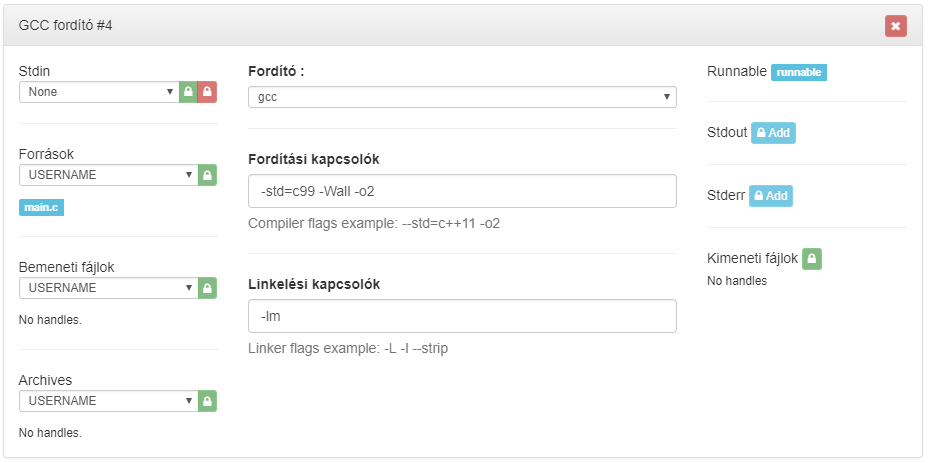
\includegraphics[]{exercise_blokk.png}
    }
    \caption{GCC fordító blokk adminisztrációs felülete}
    \label{fig:exercise_blokk}
\end{figure}

A beadás végső eredménye egy speciális blokk értéke lesz. Ennek a SubmissionResult blokknak egy bemente van, mely ha igaz a beadás sikeresnek tekinthető, ellenkező esetben sikertelen.

A blokkok kiértékelése (hasonlóan \aref{section:dynamic_dependencies}. pontban leírtakhoz) egy függőségi gráf felépítésével kezdődik, melynek kezdőpontja a fentebb említett SubmissionResult blokk. Csak azok a blokkok kerülnek kiértékelésre, amelyek (közvetve vagy közvetlen) függnek ettől a blokktól, hiszen a többi nem befolyásolja a beadás sikerességét.  Itt sem megengedettek a körkörös függőségek, tehát az elkészült gráfnak körmentesnek kell lennie.

\section{Jogosultságkezelés a JPortában}\label{subsection:permissions}

A JPorta által használt Django keretrendszer beépítetten tartalmaz egy egyszerű jogosultság kezelő rendszert. Ez lehetővé teszi különböző jogosultságok hozzárendelését felhasználókhoz, vagy felhasználói csoportokhoz. Minden Django modellhez \cite{DjangoModel} tartozik alapértelmezés szerint három jogosultság, melyeket a keretrendszer automatikusan hoz létre. Ezek a létrehozás (add), módosítás (change) és törlés (delete) jogosultságok. Sok esetben már ezek is elegek lehetnek számunkra, de bármikor létrehozhatunk új jogosultságokat, melyekkel személyre szabottabban tudjuk kezelni a hozzáférést egy-egy funkcióhoz. Ezeknek köszönhetően alapvteően egyszerűen kezelhetjük a jogosultságok kérdését \cite{DjangoAuth}. Fontos megjegyezni, hoyg Django-ban a \textit{superuser}-nek jelölt felhasználók automatikusan rendelkeznek minden jogosultsággal.

A JPorta ezen felül egyedi megoldást alkalmaz az egyes objektum példányok elérésének szabályozására, mely az access control list (ACL, \cite{ACL}) technikához hasonló. Az ACL minden objektumhoz rendel egy mátrixot, mely oszlopaiban a személyek (actor), soraiban pedig az egyes műveletek (action) találhatóak. Egy személy akkor hajthat végre egy műveletet, ha a mátrix általa és a művelet által meghatározott cellája igaz értéket tartalmaz.

\Aref{fig:acl}. ábra egy ilyen példát szemléltet: az objektumhoz tartozó hozzáférési mátrix értelmében Bob-nak csak olvasási, Alice-nak pedig olvasási és írási joga van. Emiatt Alice mind az olvasási, mind az írási műveletet sikeresen végrehajthatja, Bob azonban írási műveletet nem hajthat végre.

\begin{figure}[h]
    \centering
    \resizebox{\textwidth}{!}{
        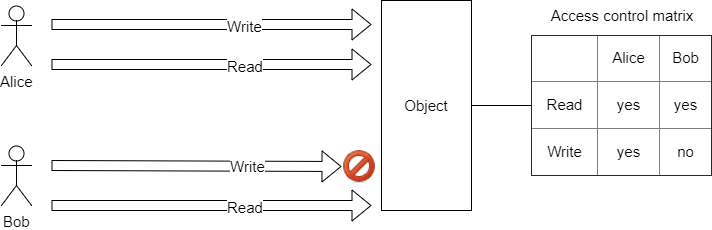
\includegraphics[]{ACL.png}
    }
    \caption{ACL működése és egy hozzáférési mátrix}
    \label{fig:acl}
\end{figure}

A portál közvetlen jogosultságok helyett jogosultsági szinteket használ, tipikusan tulajdonosi (owner) és operátori (operator) szintekkel, de ez modellenként eltérő lehet. Ilyenkor ha egy felhasználót egy objektum tulajdonosának jelölünk, egyben operátori jogosultságokkal is felruházzuk. Ha egy felhasználónak nem kívánunk jogosultságot adni az adott objektumhoz, akkor nem jelöljük egyik szinten sem. Fontos megjegyezni, hogy a \textit{superuser}-nek jelölt felhasználók itt is automatikusan rendelkeznek minden jogosultsági szinttel.

Ez a megoldás kifinomultabbnak mondható az eredeti ACL technikához képest, mivel így különböző műveletek halmazát rendelhetjük egy adott szinthez, pl. az operátor jogosult megtekinteni és módosítani az adott objektum tulajdonságait, de a törléshez már tulajdonosi szintre van szükség.

\section{Jogosultságkezelés felülvizsgálata}

Az automatikus kiértékelő modulnál a jogosultság kezelés korábban nem készült el megfelelően, így ugyan hallgatói oldalról nézve minden jól működött, a feladatokat csak \textit{superuser} jogokkal rendelkező adminisztrátorok hozhatták létre. Ez pedig nagyban megnehezítette felsőbbéves hallgatók, laborvezetők bevonását a rendelkezésre álló feladatok bővítésére. Ennek oka, hogy ekkor minden más adatot is láttak volna a portálon, beleértve minden hallgató eredményeit, megoldásait, ami nem megengedhető.

Ezek értelmében a jogosultság kezelés kibővítésével a cél az volt, hogy egyszerűen és biztonságosan lehessen automatikusan kiértékelődő feladatok létrehozására és szerkesztésére. Az így elkészült rendszer alkalmazza mindkét fenti hozzáférés szabályozási módszert a maximális biztonságos elérésének érdekében.

Először is módosítottam a meglévő szerkezetet úgy, hogy 

Author fájlok védelme

\section{Kód lefedettség ellenőrzés}

\section{Feladatok (tesztek) importálása és exportálása}

\section{Feladatok csoportosítása}

\section{További lehetőségek}

\subsection{Plágiumkeresés}

\subsection{Verziókezelő támogatás}